\begin{frame}

\begin{itemize}
    \item Flexible Neural Machine Translation Architecture Combination
    \item Related Work
    \item \emph{\color{UOYellow}Experiments}
    \item Conclusion
\end{itemize}

\end{frame}

\begin{frame}
    \begin{columns}
        \begin{column}{0.55\paperwidth}
            \frametitle{Experiments: Setup}
            \begin{itemize}
                \item Used adapted version of SOCKEYE (Heiber et al. 2017)
                \item Used WMT and IWSLT datasets for different sets of text, which are
                    on the order of 5 million training sentences.
                \item English $\rightarrow$ German and Latvian $\rightarrow$ English
                    translation problems.
                \item Ran each experiment 3 times with different random seeds. values
                    reported are the mean result and standard deviation of the BLEU and
                    METEOR scores.
            \end{itemize}
        \end{column}
        \begin{column}{0.4\paperwidth}
            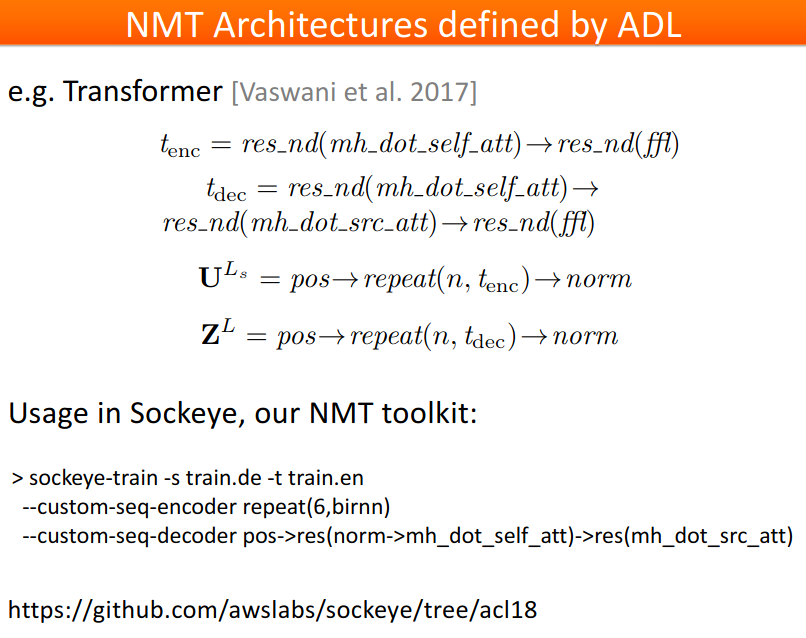
\includegraphics[width=\textwidth]{Sockeye.png}
        \end{column}
    \end{columns}
\end{frame}

\begin{frame}
    \frametitle{Experiments: What to Attend To?}
    \begin{columns}
        \begin{column}{0.55\paperwidth}
            \begin{itemize}
                \item Best attention on the upper encoder block. 
                \item No gains observed by attention on different encoder layers
                    in source attention mechanism.
            \end{itemize}
        \end{column}
        \begin{column}{0.4\paperwidth}
            \vspace{-1em}
            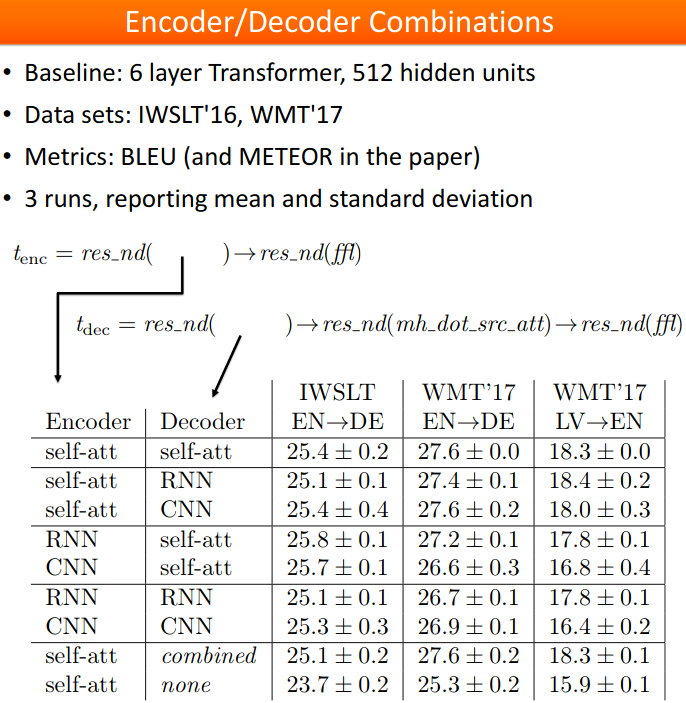
\includegraphics[width=\textwidth]{EncoderDecoder.png}\\
            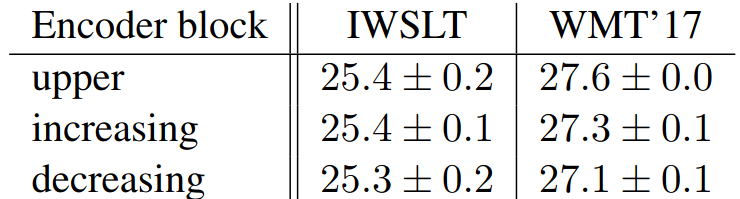
\includegraphics[width=\textwidth]{BLEUScores.png}\\
            \vspace{-1.5em}
            \center{BLEU Scores}
        \end{column}
    \end{columns}
\end{frame}

\begin{frame}
    \frametitle{Experiments: Network Structure\\\small{\vspace{-1.5em}RNN
    $\mapsto$ Transformer}}
    \begin{columns}
        \begin{column}{0.55\paperwidth}
            \vspace{-1em}
            \begin{itemize}
                \item RNN includes multiple source attention layers,
                    multi-headed attention, layer normalization, residual
                    upscaling FF layers, and single headed MLP attention.
                \item Start with RNN, add multi-headed attention (mh),
                    positional embedding (pos), layer normalization (norm),
                    single headed attention, attention to residual blocks 
                    (multi-att), and residual feed-forward layers after
                    attention blocks (ff).
                \item Gains from multi-headed attention and feed-forward
                    residual layers.
            \end{itemize}
        \end{column}
        \begin{column}{0.4\paperwidth}
            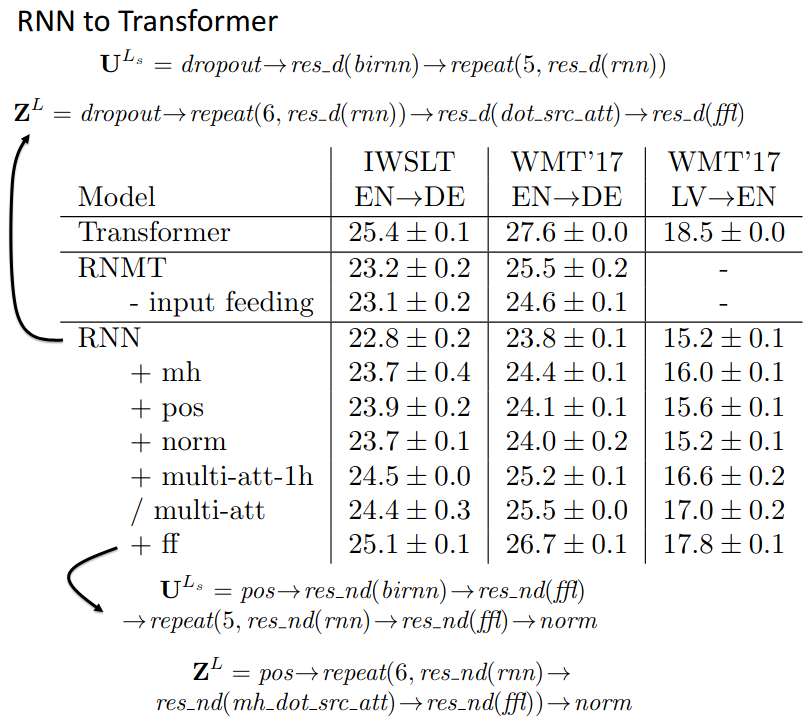
\includegraphics[width=\textwidth]{RNN2Trans.png}
            Can see that as RNN $\mapsto$ Transformer the BLEU scores increase.
        \end{column}
    \end{columns}
\end{frame}

\begin{frame}
    \frametitle{Experiments: Network Structure\\\small{\vspace{-1.5em}CNN
    $\mapsto$ Transformer}}
    \begin{columns}
        \begin{column}{0.55\paperwidth}
            \begin{itemize}
                \item Neither Transformer nor CNN have dependency between
                    decoder timesteps during traning, use multiple source
                    attention mechanisms, and use different residual structures.
                \item Largest gains from adding residual feed-forward layers. 
            \end{itemize}
        \end{column}
        \begin{column}{0.4\paperwidth}
            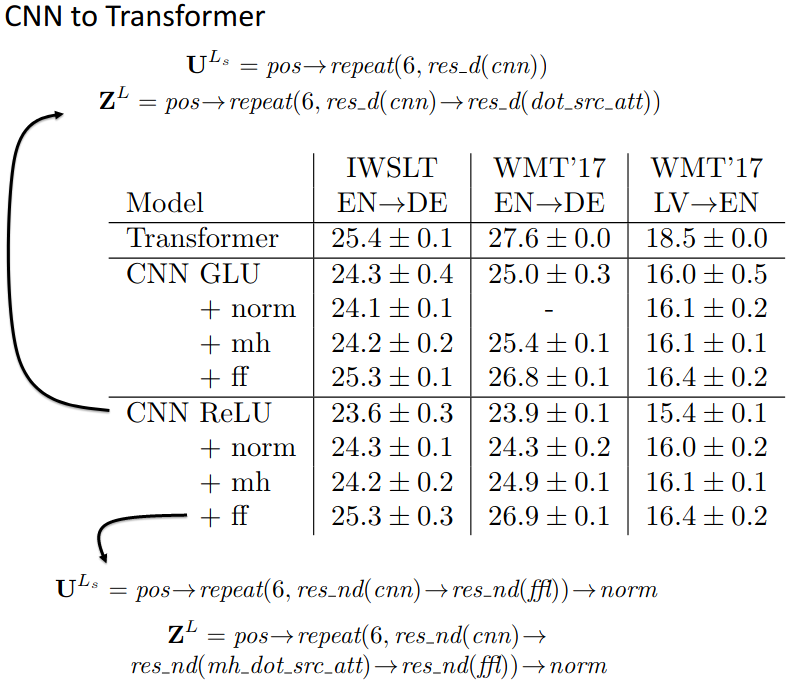
\includegraphics[width=\textwidth]{CNN2Trans.png}
            Can see that as CNN $\mapsto$ Transformer the BLEU scores increase.
        \end{column}
    \end{columns}
\end{frame}

\begin{frame}
    \frametitle{Experiments: Self-Attention Variations}
    \begin{itemize}
        \item Self-attention has advantage because two positions directly
            connected and no dependencies between consecutive timesteps.
        \item Self-attention has disadvantage because positional information
            isn't directly represented and need multiple heads.
        \item Experiments show attention is more important to decoder side.
        \item Attention on encoder shows little to no improvement.
    \end{itemize}
\end{frame}

\begin{frame}
    \frametitle{Experiments: Self-Attention Variations}
    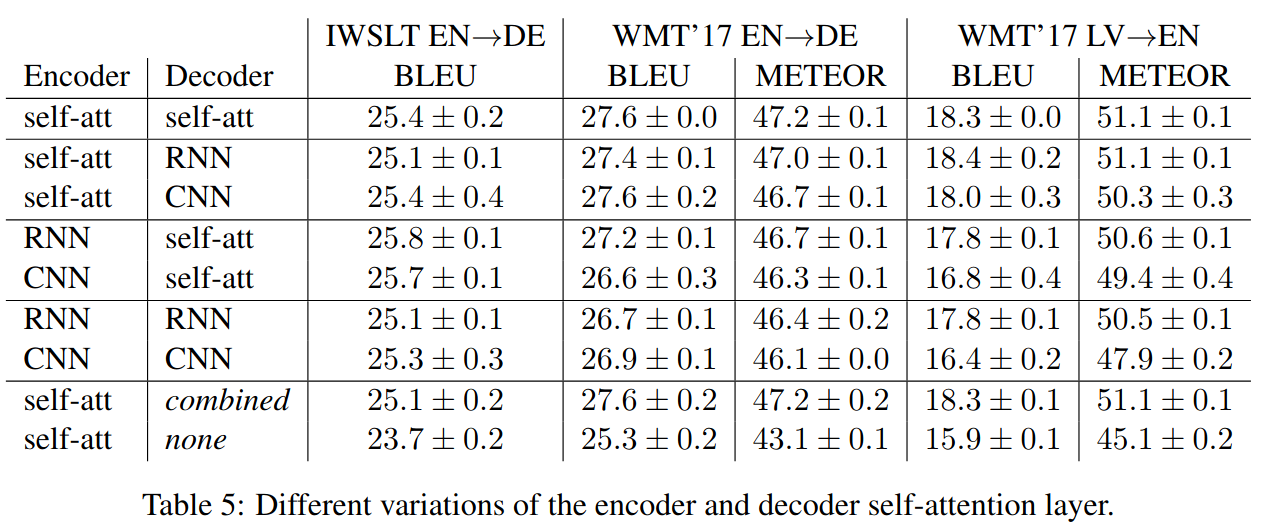
\includegraphics[width=\textwidth]{Variations.png}
\end{frame}
